\chapter{Contesto applicativo }
--Aggiungere motivazioni del lavoro, stato  dell’arte della geolocalizzazione indoor e quali problemi si vogliono risolvere-- \\

\section{Context-aware computing}
\label{context-aware}
Il sistema realizzato nell'ambito di questa tesi, si colloca nel paradigma di computazione noto come \textit{Context-aware computing}, ovvero un'applicazione nel quale i servizi utilizzano informazioni relative al contesto. In \cite{context} si definisce come \textit{context}:

\begin{quotation}
\textit{Ogni informazione che può essere usata per caratterizzare la situazione di un'entità. Ovvero una persona, un posto o un oggetto che è considerato rilevante all'interazione tra l'utente e l'applicazione, inclusi quest'ultimi.}
\end{quotation}

Questa definizione facilita il lavoro di progettazione e sviluppo di un applicazione permettendo di identificare quali informazioni sono importanti e quali no.
Consideriamo un'applicazione nel quale l'utente deve registrare il peso degli oggetti presenti nel magazzino tramite una bilancia come mostrato nella figura seguente:

\begin{figure}[H]  
	\centering 
	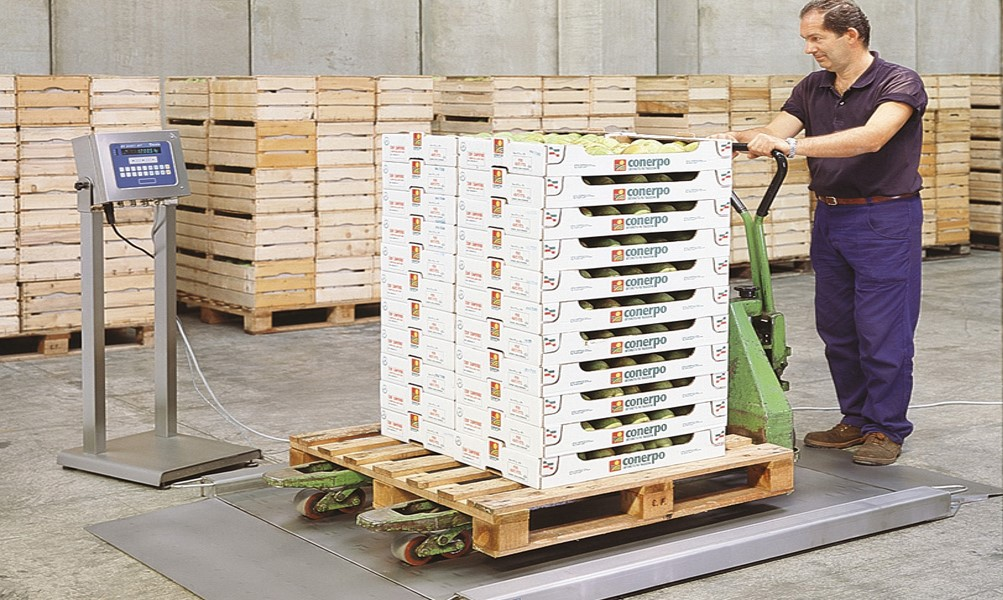
\includegraphics[scale=0.4 ]{ContestoApplicativo/bilancia.jpg}
	\caption{Esempio esplicativo del concetto di contesto}
	\label{fig:context}
\end{figure}
Nello scenario descritto le \textit{entità} sono rispettivamente utente e sistema, mentre due possibili informazioni riguardanti il contesto sono la presenza di altre persone e la posizione geografica del magazzino.\\
La presenza di altre persone nelle vicinanze non influisce il compito dell'utente, quindi non può essere considerato come informazione contestuale. La posizione geografica del magazzino invece lo è, infatti se questo fosse situato in Italia il peso verrebbe calcolato in chilogrammi mentre se fosse situato negli USA verrebbe calcolato in libbre.\\
I sistemi che reperiscono, usano o interpretano queste informazioni contestuali sono detti \textit{context-aware} e vengono definiti in \cite{context} come:
\begin{quotation}
	\textit{Un sistema è context-aware se usa il contesto per fornire informazioni rilevanti e/o servizi agli utenti, dove la rilevanza dipende dal compito degli utenti.}
\end{quotation}
Uno dei tipi di context-aware più utilizzati si basa sul contesto della localizzazione, ovvero servizi basati sulla conoscenza di dove qualcosa o qualcuno si trovi. Nell'era moderna i servizi basati sulla localizzazione (in inglese: Location based services LBSs) stanno assumendo sempre più importanza nelle attività quotidiane dell'uomo, grazie anche alle molteplici possibili applicazioni, tra i quali navigazione assistita per autoveicoli, tracking di persone sensibili (bambini, anziani, malati), servizi di emergenza e così via.\\
I LBSs vengono divisi in due macro categorie:
\begin{itemize}
	\item \textbf{OPSs}: Outdoor Positioning System Service, ovvero servizi di localizzazione in ambienti aperti.
	\item \textbf{IPSs}: Indoor Positioning System Service, ovvero servizi di localizzazione in ambienti indoor.
\end{itemize}
La tecnologia satellitare nota come Global Positioning System (GPS) è la tecnologia dominante negli OPSs. Attraverso una rete dedicata di satelliti artificiali in orbita, fornisce ad un terminale mobile o ricevitore GPS informazioni sulle sue coordinate geografiche ed orario, in ogni condizione meteorologica, ovunque sulla Terra o nelle sue immediate vicinanze ove vi sia un contatto privo di ostacoli con almeno quattro satelliti del sistema. La localizzazione avviene tramite la trasmissione di un segnale radio da parte di ciascun satellite e l'elaborazione dei segnali ricevuti da parte del ricevitore \cite{gps}.\\ 
Il grande limite di questa tecnologia è che i ricevitori devono essere nella line of sight (letteralmente a vista d'occhio) di almeno quattro satelliti nel cielo, questo significa che all'interno di edifici e spazi chiusi il segnale viene attenuato e i sistemi perdono di accuratezza. Quindi la tecnologia GPS non è adatta ai servizi di localizzazione indoor.\\
Il sistema realizzato nell'ambito di questa tesi si colloca nell'ambito degli IPSs approfonditi nel paragrafo successivo.


\section{Indoor Positioning System Service}
Un sistema di posizionamento indoor (in inglese: Indoor positioning system o IPS) è un sistema in grado di localizzare \textit{oggetti} o \textit{persone} all'interno di edifici utilizzando onde radio, campi magnetici, segnali acustici e/o altre informazioni raccolte dai sensori all'interno di dispositivi mobili \cite{IPS} o da altri  appositamente installati nell'ambiente. Questi sono una specializzazione dei più generici sistemi \textbf{RTLS}, standardizzati dall'\textit{International
Organization for Standardization and the International Electro Technical Commission} (ISO/IEC 24730). Lo standard definisce i sistemi RTLS come:
\begin{quotation}
	\textit{“ I Real time locating system sono sistemi wireless con l'abilità di localizzare la posizione di oggetti ovunque essi siano in uno spazio definito in un certo momento che è, o si avvicina, real time. La posizione è derivata dalla misurazione delle proprietà fisiche del collegamento radio."}
\end{quotation}
La differenza tra RTLS e IPS è che i primi sono stati pensati per le compagnie che vogliono tracciare i propri oggetti e le persone, fornendo uno storico di dove sono stati e dove si trovano ora. Mentre gli IPS sono pensati per essere utilizzati da utenti su dispositivi mobili per navigare ed orientarsi all'interno di edifici.
Come già accennato, gli IPS \cite{IPS2} permettono di creare una vasta gamma di servizi, ad esempio:
\begin{itemize}
	\item\textbf{ Way-Finding}: permettere di navigare in edifici complessi, come ad esempio aeroporti, seguendo il percorso indicato.
	\item\textbf{ Ricerca dei punti d'interesse}, aumentare la customer experience facendo trovare all’utente ciò che desidera.
	\item \textbf{Multi-Dot}: visualizzare in una mappa le posizioni degli utenti per tracciare persone potenzialmente in pericolo (bambini, anziani).
	\item \textbf{Marketing di prossimità}: realizzare marketing mirati, inviando annunci sulle ultime offerte.
\end{itemize}
L’elenco di cui sopra rappresenta solo un ridotto sottoinsieme dei potenziali campi applicativi (vedi Fig.\ref{fig:surveyApplication}), per questo motivo negli ultimi anni \cite{indoorThesis} l'interesse nella ricerca e nello sviluppo di sistemi di questo tipo è cresciuto sempre più tra le aziende, che hanno percepito la possibilità di grandi profitti in un mercato non ancora esplorato del tutto.
\begin{figure}[H]  
	\centering 
	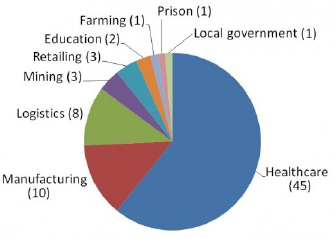
\includegraphics[scale=1.2]{ContestoApplicativo/application.png}
	\caption{Sondaggio tra 74 casi di studio di applicazioni IPS \cite{market}}
	\label{fig:surveyApplication}
\end{figure}

Secondo un sondaggio  di \textit{Markets and Markets} e un articolo pubblicato da\textit{ The International News Magazine}, il mercato degli IPS subirà una crescita annuale media del 42.1\% arrivando a valere 2.60 bilioni di dollari nel 2018. Questo da un'idea del perché grandi aziende come Google, Sony, Microsoft e Apple stiano investendo in questo settore.\\
Un'ulteriore spinta è data dal fatto che, al contrario del GPS per gli OPS (vedi \ref{context-aware}), tuttora non esiste uno standard di riferimento per gli IPS. Infatti sul mercato sono disponibili diversi tipi di IPS commerciali che si differenziano in base al principio di funzionamento e alle tecniche utilizzate, utilizzando hardware specifico o la combinazione di più sistemi.\\ 




\section{Metodi di stima della distanza}
\label{metodi_distanza}
Gli IPS possono essere classificati sulla base di diversi fattori, uno di questi è su come determinano la distanza tra due nodi.\\
Stimare \cite{IPS2} la distanza tra dispositivi wireless è utile perché attraverso questa informazione è possibile determinarne (con un certo errore) la posizione rispetto ad un sistema di riferimento. I metodi che permettono di stimare la distanza emettitore-ricevitore [\cite{alg1}, \cite{alg2}]si distinguono in:

	\begin{itemize}
	\item \textbf{Range based}:
	
		\begin{itemize}
		\item \textit{RSSI}- potenza del segnale radio ricevuto(sez.\ref{rssi})
		\item \textit{ToA} - tempo d’arrivo: (sez.\ref{toa})
		\item \textit{TDoA} - differenze del tempo di arrivo (sez.\ref{tdoa});
 	    \end{itemize}
     
	\item \textbf{Angle based}:
		\begin{itemize}
			\item \textit{AoA} - Angle of Arrival (sez.\ref{aoa}).
		\end{itemize}
		
\end{itemize}
Per poter determinare le distanze si devono distinguere i punti di riferimento (che hanno
delle coordinate note) dai nodi senza posizione nota a cui assegnare delle coordinate.
Si dicono:
\begin{itemize}
	\item \textbf{Anchor}: i nodi le cui coordinate sono note
	\item \textbf{Unknown}: i nodi di cui non si conosce la posizione.
\end{itemize}

 L’obiettivo del posizionamento è assegnare le giuste coordinate agli Unknown rispetto ad un sistema di riferimento. Questo è strettamente legato all'implementazione dell'IPS e così anche la codifica delle posizioni all'interno del sistema di riferimento, le coordinate potrebbero essere restituite all'utente in maniera relativa ("vicino alla cucina") oppure assoluta ("tre  metri in direzione ovest dal nodo 1").

\subsection{Stime della distanza Range based}
Nel posizionamento dei nodi basato sulla distanza la stima della posizione del target dipende dai seguenti parametri:
	\begin{itemize}
	\item il tempo trascorso tra l’emissione e la ricezione del segnale radio;
	\item la distanza euclidea tra ogni emettitore ed il ricevitore;
	\item la potenza del segnale ricevuto.
\end{itemize}
In alcuni casi sono necessarie tre o più Anchor per ottenere le coordinate da assegnare allo Unknown.

\subsubsection{Received Signal Strength Indicator - RSSI}
\label{rssi}
La comunicazione \cite{IPS2} tra dispositivi wireless (senza fili) avviene tramite lo scambio di segnali propagati nell’aria. Durante la propagazione i segnali tendono ad attenuarsi con l'aumentare della distanza percorsa fino a non essere più percepibili.

\begin{figure}[H]  
	\centering 
	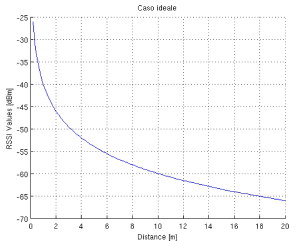
\includegraphics[scale=1.2]{ContestoApplicativo/signal.PNG}
	\caption{RSSI - Andamento della potenza in funzione della distanza percorsa dal segnale}
	\label{fig:signal}
\end{figure}

La stima della potenza del segnale ricevuto è data dall’indicatore RSSI \cite{rssi}. La distanza emettitore-ricevitore si stima utilizzando \textbf{l’equazione di trasmissione di Friis}.

\begin{equation}
		P_{T}=P_{R} \dfrac{G_{T}G_{R}\lambda^2}{(4\pi)^2d^n}
		\label{eq1}
\end{equation}

dove:
\begin{itemize}
	\item $P_{R}$: potenza del segnale ricevuto (Watt)
	\item $P_{T}$: potenza del segnale trasmesso(Watt)
	\item $G_{R}$: guadagno dell'antenna ricevente
	\item $G_{T}$: guadagno dell'antenna trasmittente
	\item $\lambda=\frac{v}{f}$: lunghezza d'onda, dove $v$ è la velocità di propagazione e $f$ è la frequenza dell'onda
	\item $d$: distanza espressa in metri
	\item $n$: constante di propagazione del segnale che dipende dall'ambiente 
\end{itemize}

Con la seguente equazione invece è possibile convertire la potenza espressa in Watt nella potenza espressa in dBm:
\begin{equation}
P[dBm] = 10\log_{10}(10^3P[W])
\label{eq2}
\end{equation}
Combinando l'equazione \ref{eq1} con \ref{eq2} e applicando le proprietà dei logaritmi si ottiene:
\begin{equation}
RSSI = -(10 n \log_{10} d - A)
\label{eq3}
\end{equation}
dove $A$ è la potenza del segnale ricevuto a distanza fissa di un metro (espressa in dBm), considerando una costante di propagazione $n$.\\
La stima della distanza si ottiene infine dalla seguente equazione:
\begin{equation}
d = 10 (\frac{A - RSSI}{10n})
\label{eq4}
\end{equation}
Tuttavia la distanza restituita non è del tutto precisa, infatti la potenza del segnale potrebbe essere alterata dall'ambiente circostante attraverso i fenomeni di \textbf{Riflessione} (il segnale sbatte e si riflette su vari ostacoli seguendo più percorsi) e di \textbf{Assorbimento} (il decadimento viene alterato dagli oggetti presenti). Tale tecnica viene solitamente completata utilizzando il metodo della \textbf{Trilaterazione} (sez.\ref{trilaterazione})\\


\subsubsection{Time Of Arrival measurements}  
\label{toa}
A differenza del precedente metodo, con questa tecnica la distanza tra emettitore e ricevitore viene stimata sulla base del tempo impiegato dal segnale a raggiungere il ricevitore. Nello specifico la sequenza di azioni è:
\begin{enumerate}
	\item Il nodo \textit{A} invia il segnale al tempo $t_1$
	\item Il segnale arriva al nodo \textit{B} al tempo $t_2$
	\item \textit{B} elabora il messaggio impiegando un tempo $t_d$ e lo invia al tempo $t_3$
	\item Il segnale torna al nodo \textit{A} al tempo $t_4$
\end{enumerate}
Come mostrato dalla figura seguente:

\begin{figure}[H]  
	\centering 
	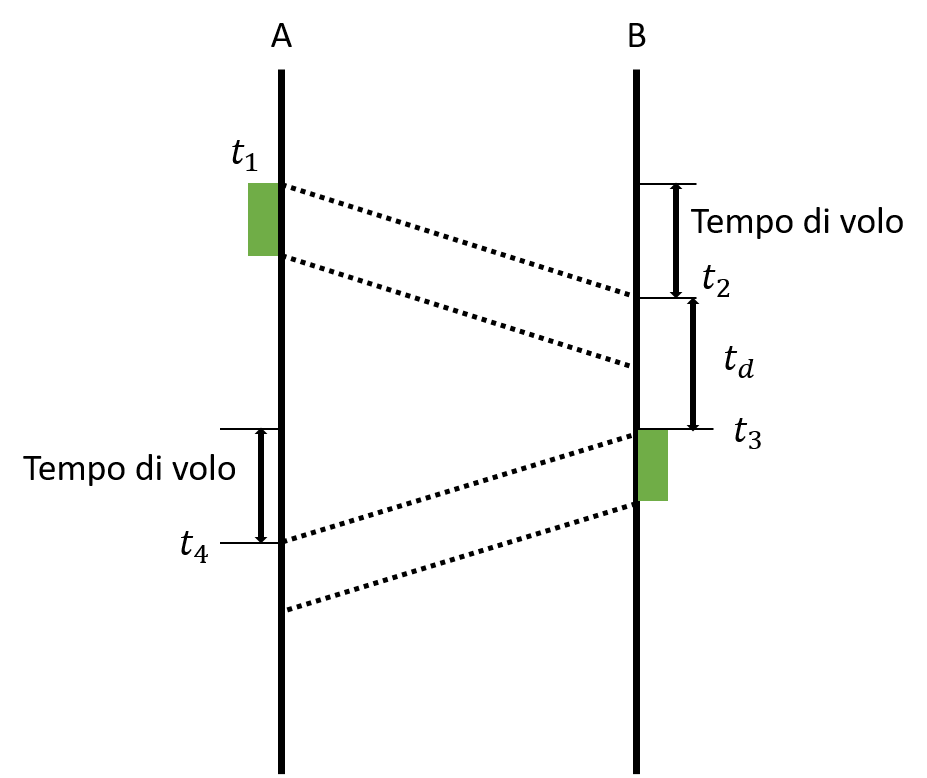
\includegraphics[scale=0.4]{ContestoApplicativo/toa.png}
	\caption{ToA - Principio di funzionamento}
	\label{fig:toa}
\end{figure}

Quindi il tempo di viaggio può essere ricavato con la seguente equazione:

\begin{equation}
t_d = \dfrac{(t_4 - t_1) - (t_3 - t_2)}{2}
\label{td}
\end{equation}

E infine la distanza stimata attraverso:
\begin{equation}
d_{ToA} = t_d * c
\label{eq:toa}
\end{equation}

dove $c$ è la velocità di propagazione della luce nel vuoto pari a 299792458 m/s. Questa tecnica viene solitamente completata dalla tecnica di trilaterazione (sez. \ref{trilaterazione}) come per le misure RSSI viste precedentemente. I sistemi che usano questa tecnica generalmente hanno bisogno un complesso meccanismo di sincronizzazione per mantenere una fonte affidabile di tempo per i sensori\cite{toaProblem}

\subsubsection{Time Difference Of Arrival}
\label{tdoa}
E' una versione migliorata del ToA(sez.\ref{toa}). Permette di 



\begin{figure}[H]  
	\centering 
	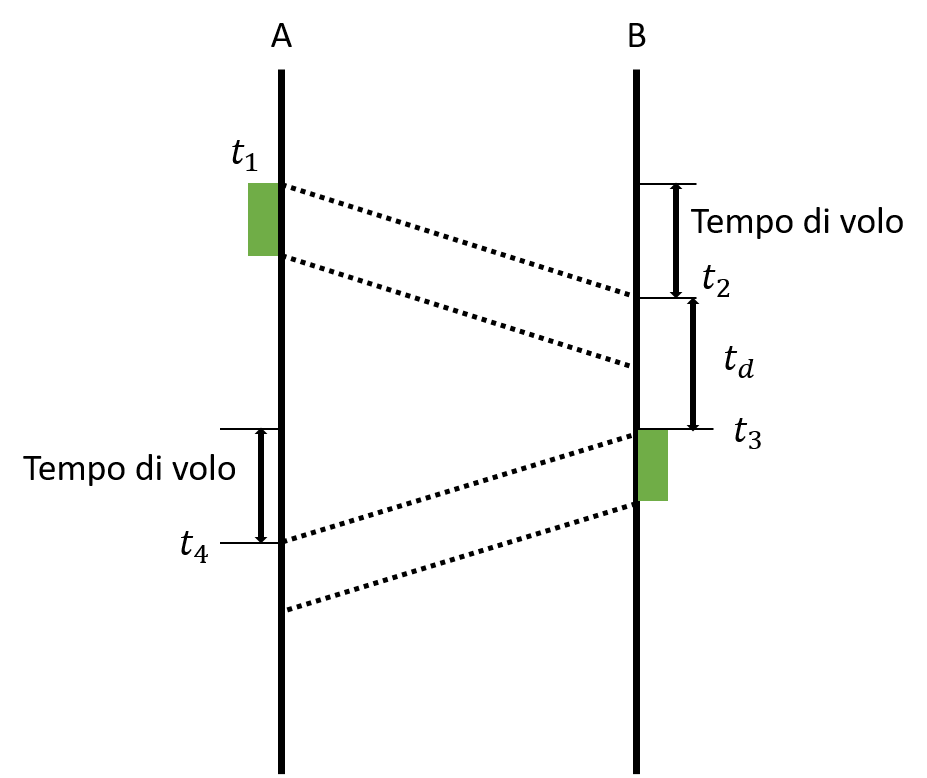
\includegraphics[scale=0.4]{ContestoApplicativo/toa.png}
	\caption{TDoA - Principio di funzionamento}
	\label{fig:tdoa}
\end{figure}






\section{Metodi di posizionamento}


\subsection{Trilaterazione}
\label{trilaterazione}
Consideriamo 3 \textit{Anchor} intorno cui disegniamo 3 circonferenze aventi per centro le coordinate degli \textit{Anchor} e per raggio l'RSSI del segnale ricevuto dallo \textit{Uknown}, come mostrato in figura:
\begin{figure}[H]  
	\centering 
	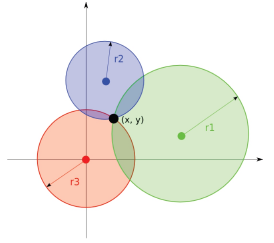
\includegraphics[scale=0.8]{ContestoApplicativo/trilaterazione.png}
	\caption{Trilaterazione - Esempio esplicativo}
	\label{fig:trilaterazione}
\end{figure}
Quindi le coordinate dell'Unknown sono la soluzione del seguente sistema:
\begin{equation}
\begin{cases}
(x-x_1)^2 + (y-y_1)^2 = r_1^2\\
(x-x_2)^2 + (y-y_2)^2 = r_2^2\\
(x-x_3)^2 + (y-y_3)^2 = r_3^2
\end{cases}
\end{equation}
Essendo un sistema 









